\section{Lemmatization and part-of-speech tagging}
\label{chap:tag}
Lemmatization and \acrlong{pos} tagging tasks are categorized as morphological analysis, shares same architecture and trained network and they will be described together in this section.
\subsection{Task Definition}
%co chci presne delat - vstup, vystup, metrika

\paragraph{\textbf{POS tagging}} \mbox{}\\
\textit{input}: a sequence of  words \\
\textit{output}: tag (for each word), which contains not only part-of-speech (e.g. noun, pronoun, punctuation mark) but also other morphological analysis (case, tense, etc) corresponding to 15-places morphological tagging system by \cite{Hajic2004}. Description of each position can be found in Table \ref{Tab:tagset}. %For more detailed  description or for exploration of predictions given by this work is recommended to use website of Institute of Theoretical and Computational linguistics \footnote{http://utkl.ff.cuni.cz/~skoumal/morfo/?pos=11&val=1}.

\paragraph{\textbf{Lemmatization}} \mbox{}\\
\textit{input:} a sequence of words \\
\textit{output:} lemma -- a base form of a given words, for example nominative of singular for nouns or infinitive for verbs. In this work, lemmatization is treated as a classification problem with classes coresponding to generating rules which transform an input word into target lemma. For example of such rules see Figure \ref{fig:lemma_rules}. \\ %TODO kolik jich je v datasetu

\begin{table}[!ht]
\centering
\begin{tabular}{ |c|c|c| } 

 \hline
 Position & Name & Description \\ 
 \hline \hline
 1 & POS & Part of speech \\ \hline
 2 & SubPOS & Detailed part of speech \\ \hline
  3 & Gender & Gender \\ \hline
4 & Number & Number \\\hline
  5 & Case & Case \\ \hline
 6 & PossGender & Possessor's gender \\\hline
  7 & PossNumber & Possessor's number \\ \hline
8 & Person & Person \\\hline
  9 & Tense & Tense \\ \hline
 10 & Grade & Degree of comparison\\\hline
  11 & Negation & Negation \\ \hline
 12 & Voice & Voice \\\hline
 13 & Reserve1 & Reserve \\ \hline
14 & Reserve2 & Reserve \\\hline
  15 & Var & Variant, style \\ 
 \hline

\end{tabular}
\caption{Czech morphology developement is dated from 1989 \citep{Hajic2004} 
and in description of words uses 15-places morphological tags as described in this table taken from \url{https://ufal.mff.cuni.cz/pdt2.0/doc/manuals/en/m-layer/html/ch02s02s01.html}. For more detailed  description or for exploration of predictions given by this work is recommended to use website of Institute of Theoretical and Computational linguistics: http://utkl.ff.cuni.cz/~skoumal/morfo/?pos=11\&val=1}
\label{Tab:tagset}
\end{table}

%the longest common substring between the form and the lemma, and then compute the shortest edit script converting the prefix and suffix of the form into the prefix and suffix of the lemma using the Wagner–Fischer algorithm (Wagner and Fis- cher, 1974). Upon predicting a lemma edit script, we apply the edit operations to the word form to produce the final lemma. z kondraytuk


\paragraph{Metric} used for evaluation of the model is an accuracy reported separately for several options -- only tags/lemmas, accuracy of joint classification of tags and lemmas, and  also for all three variants with an usage of a morphological dictionary (this option is described in more detail in \ref{sub:dataset}).

\begin{figure}[H]
\centering
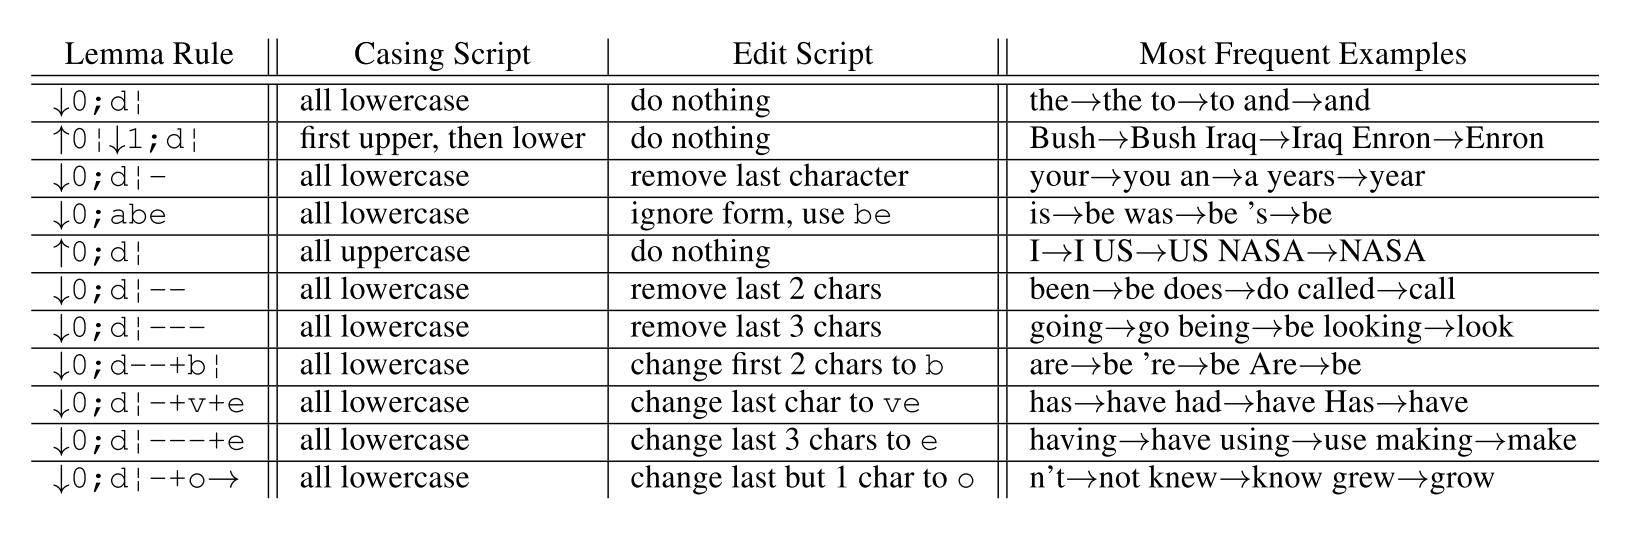
\includegraphics[width=1\textwidth]{../img/lemma_rules}
\protect\caption{
Table 1 from \citep{Straka2019b} presents 10 most common lemma generating rules in English EWT corpus. Each rule has two parts -- casing script for transforming uppercase and lowercase letters, and edit script. Edit script can transform prefix, suffix, or also a root of the word. It uses the Wagner–Fischer algorithm \citep{Wagner}, which finds the longest commont substring between the word and its lemma. Resulting rule is the shortest edit script converting the word into the lemma. More information can be found in \citep{Straka2019b}.
}
\label{fig:lemma_rules}
\end{figure}


\subsection{Related Work}
\subsubsection{Tagging}
\paragraph{Best results}
This work aims to improve previously published SOTA results for contextualized embeddings in Czech lemmatization and tagging \citep{straka2019czech} and \citep{Straka2021}. POS tagging (for English) is dated back to 1971 with first rule-based approach on Brown Corpus \citep{greene1971automatic}. Good results in POS tagging were achieved after year 2000 using both classical machine learning methods like Hidden Markov Models \citep{tnt} or Support Vector Machines \citep{svmtool}, and perceptrons/neural networks \citep{collins-2002-discriminative}. Actual \acrlong{sota} known to me is presented in Flair model \citep{Akbik2018}\footnote{More detailed overvirew can be found here: https://aclweb.org/aclwiki/}. It is necessary to note that first papers had \acrshort{pos} tagging defined differently than it is in this work. They focused only on selecting part fo speech (noun, verb etc...), meanwhile later works (including this thesis) presents complex morphological analysis. %TODO zo je zo slovo? 
One of first automatical tagging experiments in Czech is described in \citep{Hladka}, which also shows differences between languages with rich inflexion (as Czech) and ones with more simple morphology (for example English). Languages with complicated morphology has incomparably larger set of possible tags. Current \acrshort{sota} result is presented in \citep{Straka2021}, which uses Czech version of RoBERTa model -- RobeCzech. This is the model also used for some experiments in this work and, as expectated,  yields the best results. RobeCzech is based upon previous successful morphological analysis with contextual embeddings and BERT-like models \citep{Straka2019b}, \citep{Straka2019a}, \citep{Straka2019}, \citep{Straka2018} (all lastly mentioned models also achieved great results in lemmatization). %TODO zmnit morce, morphodita a udpipe

\paragraph{Tagsets}
Although tagging is mostly considered to be classification into predifined set of tags, the sets themselves can vary. Penn treebank uses a tagset of 54 different tags, which presents parts of speech and additional informations like tense or number \footnote{see: \url{https://www.sketchengine.eu/penn-treebank-tagset/}}. There are some differences between this tagset and other English datasets or taggers (e.g. TreeTagger \citep{Schmid95improvementsin} or CLAWS tagset \citep{Chapelle1988TheCA}). All English tagsets are really small comparing to languages like Czech or Turkish. As mentioned before, Czech uses 15-positioning tags, which is  natural solution for such languages. These positions can be predicted together or for each position separately. First approach creates big tagset but guarantees consistency among positions (e.g. there will be no tense for a noun or a case for a verb). In the case of separate prediction, each position can be treated as a classification problem separately, which causes problems, because the individual parts of tag are not independent. Better approach is to use sequence-to-sequence modelling \citep{Sutskever2014}, which outputs the tag as a sequence of positions and takes into account previously generated position as in \citep{malaviya-etal-2019-simple}. 

\subsubsection{Lemmatization}
Lemmatization has undergone a similar development as tagging, starting with rule-based approaches and statistical approaches \citep{Plisson}, continuing with neural networks and recently achieving good results with BERT-like models \citep{Kondratyuk2019}. 

\paragraph{Approaches}
Lemmatization is typically performed as a sequence-to-sequence model, therefore it takes a word as a sequence of characters and produces a new sequence of characters, which is the lemma.  %TODO proc je to lepsi ci horsi
Lemmatization as a classification task into edit scripts set firstly appeared in \citep{Chrupala} and more explored by \citep{2018}. Sequence-to-sequence model can be also used for production of edit rules (same rules as used in this work)\citep{chakrabarty2017context}, \citep{muller2015joint} and Yildiz2019.

%\citep{Kondratyuk2019} - contextual embeddings a finetunnig jako já, na 75 jazycích, používá spoustu regularizace, multilingual bert model in base size same as this work,  navazuje na udpipe, má výsledky na PDT!
%\citep{Straka2021} - sentiment,tagging i lemmatizace, t al jen embeddings a sentiment finetunning, jinakjdehlavne ocisla,je to aktualni sota,tak pouzit


%\citep{Horsmann} - are lstms good for pos tagging?
%\citep{Plank} - postagging with bilingual
%\citep{Toutanova2003} - tagging obousmerny, zmineno v kodraytuk, robeczech, straka i base berticlanky
%\citep{Wang2015} - tagging with bidirectional lstm
%\citep{Huang2015} - bilstm for tagging
%\citep{Collobert2011} ... preprocessing, tagging baseline

\subsection{Dataset and Preprocessing}
\label{sub:dataset}
%TODO popisje v straka2019 - dopnit
%TODO kolik je tam lemmat, tagů, celkem vet, pripadne tokenů - je v certovi1568
Dataset for these tasks is taken from data of Prague Dependency Treebank (PDT) \citep{PDT35}, version 3.5 from year 2018. %TODO kolik tamjedat
Data consists of sentences with lemmas and tags. For ambiguous words, data contain all possible analysis. For example, Czech word "psa" have one possible lemma ("pes") but two possible tags because it could be one of two possible grammatical cases -- genitive or accusative. Input data for such word looks as follows: \\
\begin{center}
psa pes NNMS2-----A---- NNMS4-----A----
\end{center}.
Data contains about %TODO kolik 
unique tags and 15k different lemma rules (the number of lemmas is significantly smaller than a number of unigue words or tags, because words with simiral morphological function have same way of creating lemma from the word, e.g. words \textit{malého} (little, accusative,  sg, m.,) and \textbf{červeného}  (red, accusative,  sg, m.,)  %TODO doplnit az mi dobehne job

Dataset was originally divided into tree parts - train, development and test, which is also used in this work. Input sentences are preprocessed as follows:
\begin{itemize}
\item white space deletion
\item splitting into sentences and words
\item mapping characters and words into numbers -- mapping  words/characters which were found in train dataset into integers (from one to the number of unique words). This means that the network has no information about words/characters which appears only in test or development dataset. All newly appeared words/characters are mapped into one same number (typically $0$) for \textit{UNK} token/character.
\item tokenization -- Tokenizer for corresponding BERT-like model transforms input words into tokens. Each word is transformed into one or more strings, which are converted into numbers. This serves as an input into BERT part of model. To creating these input embeddings, the whole sentence for each word is needed as same words can have different representation in different contexts. More information can be found in \ref{sub:tokens}.
\end{itemize}

\subsection{Experiments and Architecture}

%zminit udpipe a zminit kolik je tech lstm a tak,vsechny dimenze (do tabulky)

%For POS tagging, we applied a straightforward model in the lines of Ling et al. (2015) – first rep- resenting each word with its embedding, contextu- alizing them with bidirectional RNNs (Graves and Schmidhuber, 2005), and finally using a softmax classifier to predict the tags. z UDpipe2

%??? We perform tokenization, sentence segmentation and multi-word token splitting with the baseline UDPipe 1.2 approach. In a nutshell, input charac- ters are first embedded using trained embeddings, then fixed size input segments (of 50 characters) are processed by a bidirectional GRU (Cho et al., 2014), and each character is classified into three classes – a) there is a sentence break after this character, b) there is a token break after this char- acter, and c) there is no break after this character.

%reprezentation: tři typy embeddings - pretrained, trained, character-level a ještě berti

%TODO popisovat vice ty pravidla?

The model for lemmatization and tagging is build upon a model (and a code) for previous work on Czech NLP processing with contextual embedding \citep{straka2019czech}. 
Data preprocessing is taken over from the paper as well as the structure of a lemmatizer and a tagger network which is extended by BERT-like models, hoping for improvements. Previous work \citep{Straka2019} and \citep{Straka2018} showed that training tagging and lemmatization together in one network can be mutually advantageous, so both of these analysis are an output of one network and are trained jointly. Detailed visualisation of network architecture can be found in Figure \ref{pic:lt_arch}. \par The architecture of network can be divided into three parts -- inputs, optional \acrshort{rnn}s, classification head:
\paragraph{Inputs}
An input of the network is formed of five types -- characters (charseqs), words (charseq ids), correct responses(word ids), pretrained embeddings and possibly precomputed bert embeddings (depends on the experiment type). Before the further processing of inputs by \acrshort{rnn} cells, there are created two other types of embeddings: character-level embeddings and another word embeddings which are, in contrast to BERT and pretrained embeddings, also trained during training process.

\paragraph{RNN cells}
Characterlevel embeddings are further processed via \acrfull{gru} and all inputs (or their embeddings) are processed by recurrent part of network (specifically by \acrfull{lstm} cells).

\paragraph{Classification head(s)}
After the processing by recurrent neural networks, network employs two separate classification head, one for tagging and another for lemmatization. Both uses dense layer with tanh activation function to presented more non-linearity as used in \citep{2018} and a softmax function for obtaining the probability distribution over target classes. Lemmatization, however, presents one another change -- addition of character level data without RNN processing, which are used together with the rest of weights as an input into softmax following \citep{Straka2018}, because it leads to better performance of lemmatization in the case of shared network between both tasks.

%TODO kondraytuk bere predikci k prvnímu subwordu, jak to delam ja? 

\begin{figure}[!ht]
\centering
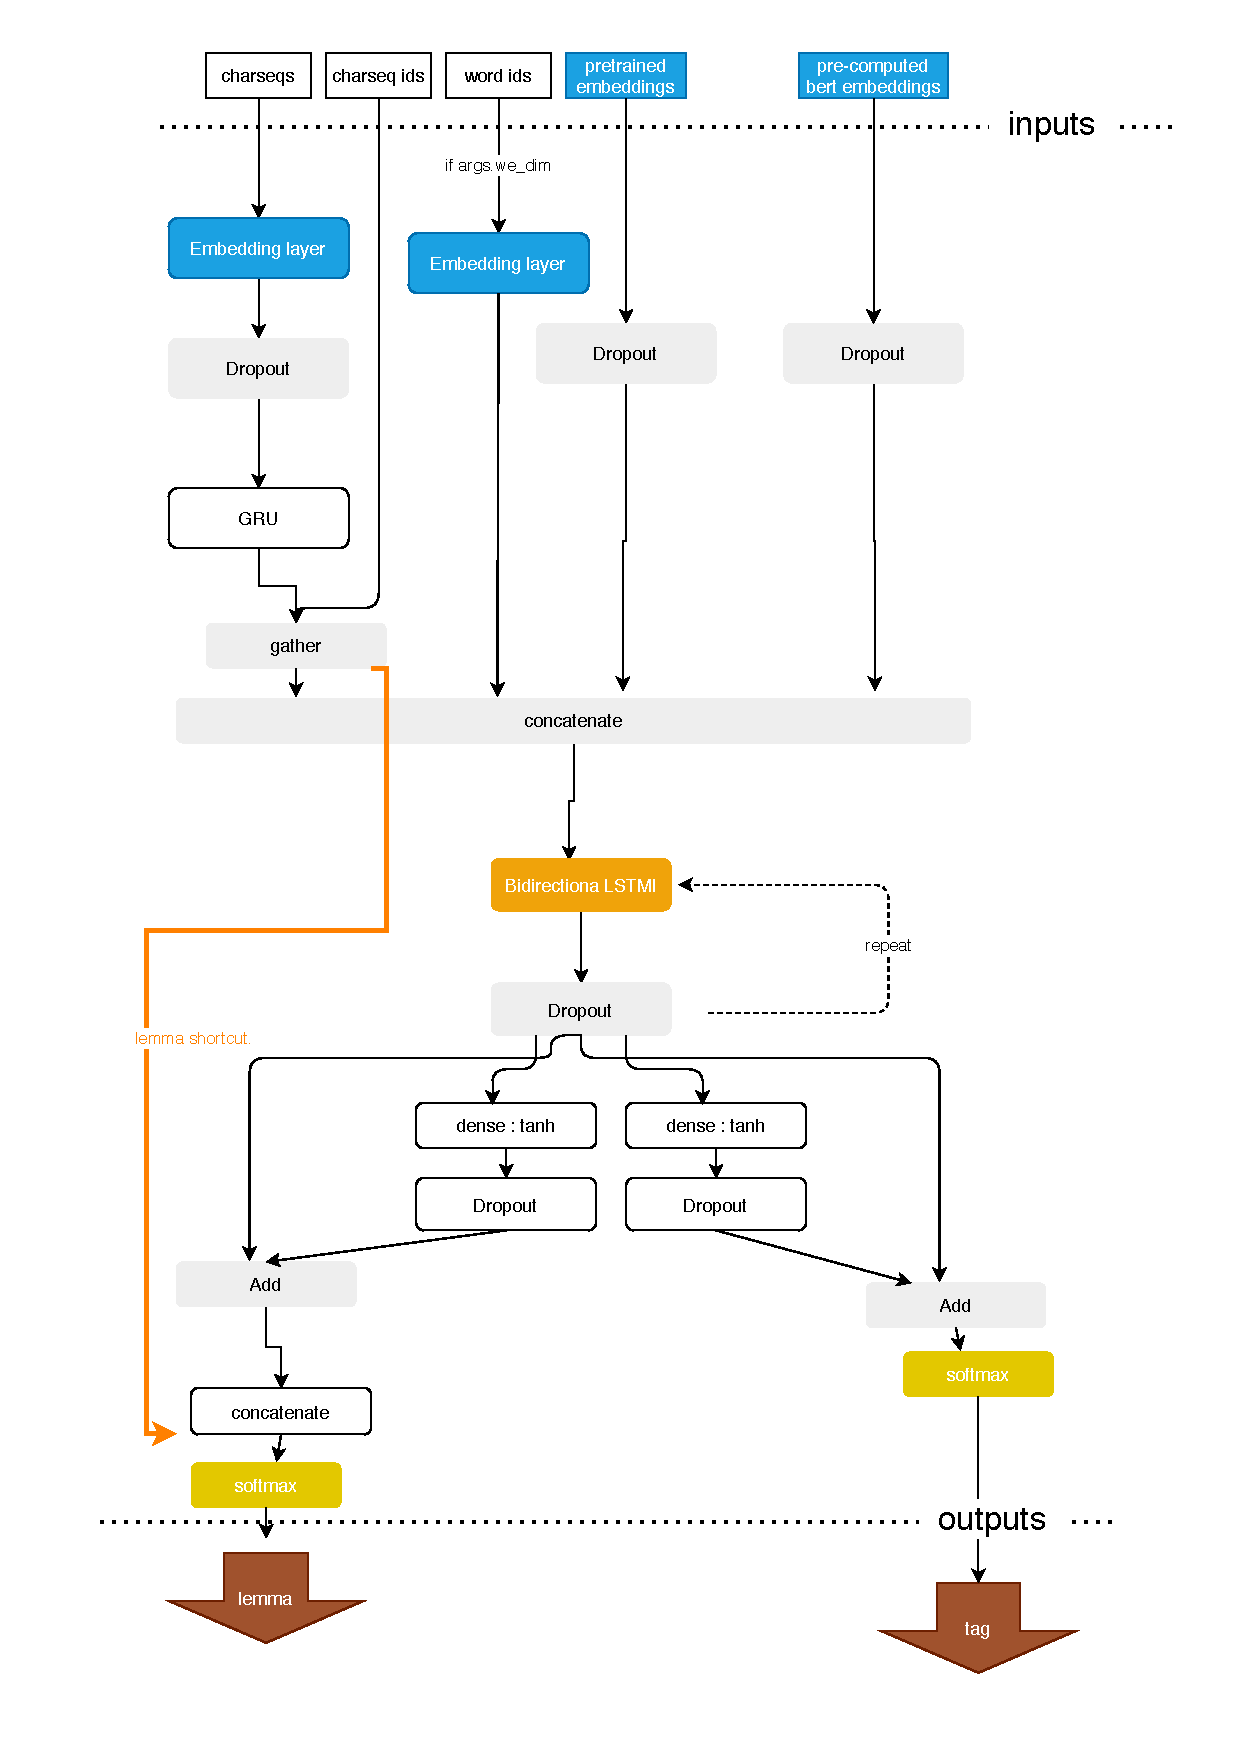
\includegraphics[width=1\columnwidth]{../img/taggermodel.pdf}
\protect\caption{popis? }
\label{pic:lt_arch}
\end{figure}

\paragraph{Morphological Dictionary} All classification can be done with or without use of a morphological dictionary MorFlex \citep{11234/1-1834}, which can provide possible pairs \textit{tag-lemma}. If so, generated tag and lemma is a pair with maximal likelihood, but chosen just from the dictionary. This leads to more consistent results. 


%TODO nekde mam taky dropouts! zminit
\subsubsection{Experiments}
This part uses all main \textbf{experiment types} as decribed in \ref{sec:expe}: \textit{base, ls, embed, fine, simple, full}. Three \textbf{BERT-like models} are used for every experiment setup:
\begin{itemize}
\item multilingual BERT (mBERT) \citep{Devlin2019} 
\item XLM-RoBERTa \citep{Conneau2019}), 
\item RobeCzech \citep{Straka2021}.
\end{itemize}
XLM-RoBERTa and mBERT are trained on 100/104 different languages including Czech and RobeCzech is recently published version of RoBERTa, trained only on Czech data. %TODO nekde v diskuzi zminit i certa,aleje horší
\textbf{Selection of layers} are made in two ways -- last four layers and learning of weighted sum of all layers. These experiment are made for finetunning setup only and as the weighted sum does not showed a significant benefit, mean of last four layer is the only method used for other experiments. %TODO je to z kondraytuk a jmenuje se to attention!
 \textbf{Learning rate} is used as usual for each type of task a and three different learning schedules were applied in each combination of hyperparameters: cosine decay \textit{(cos)}, inverted square root decay \textit{(isrd)} and a one epoch warm-up followed by a constant learning rate \textit{(warmup)}. For \textit{embed} experiments, \textit{warmup} is replaced by  a simple division of training into tow parts with different learning rates as in %TODO citace. 
Batches has size 64, given by the compromise between the pursuit of relatively big batch size and computational resources. %TODO learning rate ulmfit (warmup) a kondraytuk(inverse) 
%TODO popsat jak presne to vypada nebo alespon graficky ty learning rates
%classification head. %TODO popsat jak presne to vypada

\subsection{Results and Discussion}
%TODO jaka je baseline
%Jsou vysledky lepsi nez baseline?
%Co je nejlepší jednotlivě a celkem?
%kompletní tabulka a tabulka best z kategorií + baseline

%TODO tady upravit tabulka na nejlepší výsledky z kazde kategorie + baseline + porovnani co tam je + robeczech a o kolik procent je to lepší
\begin{table}[!h]
  \begin{tabular}{|l||c|c|c||c|c|c|}
  \hline
\multirow{2}{*}{Experiment} & \multicolumn{3}{c||}{Without Dictionary}  &
      \multicolumn{3}{c|}{With Dictionary} \\ 
    & Tags & Lemmas & Both & Tags & Lemmas & Both \\ \hline \hline
    StrakaB & 97.94\% & 98.75\% & 97.31\% & 98.05\% & 98.98\% & 97.65\% \\ \hline
    emb (lr 0.0001) &  97.80\% & 98.70\% & 97.17\% & 97.95\% & 98.93\% & 97.55\% \\ \hline
    baseline & 97.04 \% & 98.56 \% & 96.41\% &  97.31  \% & 98.83 \% & 96.90\% \\ \hline 
    StrakaC & 97.67\% & 98.63\% & 97.02\% & 97.91\% & 98.94\% & 97.51\% \\ \hline
  \end{tabular}
  \caption{%TODO cite
  Straka2019B is the best solution from \citep{Straka2019} paper. Straka2019C is a comparable solution  (BERT embeddings only), which was transformed into TF2 in this work.} 
\end{table}


\begin{table}[!ht]
\resizebox{\columnwidth}{!}{% Please add the following required packages to your document preamble:
% \usepackage{multirow}
\begin{tabular}{|l|l|l|l||llllll|}
\hline
\multicolumn{2}{|c|}{Model}                      & EXPE                    & LRTYPE & LemR & LemD & TagsR & TagsD & JointR & JointD \\ \hline \hline
0  & NA                           & base                    & simple & 98,58  & 98,81   & 97,05   & 97,31    & 96,43     & 96,9       \\ \hline
1  & NA                           & ls                      & simple & 98,55  & 98,81   & 97,12   & 97,34    & 96,51     & 96,94      \\ \hline
2  & \multirow{3}{*}{mBERT}       & \multirow{9}{*}{embed}  & simple & 98,69  & 98,93   & 97,83   & 97,98    & 97,17     & 97,58      \\ \cline{1-1} \cline{4-10} 
3  &                              &                         & cos    & 98,74  & 98,95   & 97,91   & 98,04    & 97,28     & 97,63      \\ \cline{1-1} \cline{4-10} 
4  &                              &                         & isrd   & 98,73  & 98,94   & 97,89   & 98,02    & 97,28     & 97,61      \\ \cline{1-2} \cline{4-10} 
5  & \multirow{3}{*}{xlm-Roberta} &                         & simple & 98,57  & 98,8    & 97,33   & 97,54    & 96,68     & 97,12      \\ \cline{1-1} \cline{4-10} 
6  &                              &                         & cos    & 98,6   & 98,83   & 97,45   & 97,62    & 96,81     & 97,21      \\ \cline{1-1} \cline{4-10} 
7  &                              &                         & isrd   & 98,59  & 98,83   & 97,44   & 97,61    & 96,81     & 97,2       \\ \cline{1-2} \cline{4-10} 
8  & \multirow{3}{*}{RoBECzech}   &                         & simple & 98,77  & 98,97   & 98,38   & 98,48    & 97,78     & 98,08      \\ \cline{1-1} \cline{4-10} 
9  &                              &                         & cos    & 98,79  & 98,99   & 98,38   & 98,48    & 97,8      & 98,1       \\ \cline{1-1} \cline{4-10} 
10 &                              &                         & isrd   & 98,78  & 98,98   & 98,4    & 98,48    & 97,8      & 98,09      \\ \hline
11 & \multirow{3}{*}{mBERT} & \multirow{9}{*}{fine} & simple & 98,69 & 98,93 & 97,84 & 97,99 & 97,21 & 97,59 \\ \cline{1-1} \cline{4-10} 
12 &                              &                         & cos    & 98,72  & 98,95   & 97,97   & 98,08    & 97,33     & 97,68      \\ \cline{1-1} \cline{4-10} 
13 &                              &                         & isrd   & 98,68  & 98,9    & 97,72   & 97,86    & 97,09     & 97,46      \\ \cline{1-2} \cline{4-10} 
14 & \multirow{3}{*}{xlm-Roberta} &                         & simple & 98,62  & 98,84   & 97,72   & 97,9     & 97,07     & 97,48      \\ \cline{1-1} \cline{4-10} 
15 &                              &                         & cos    & 98,67  & 98,9    & 97,95   & 98,09    & 97,32     & 97,69      \\ \cline{1-1} \cline{4-10} 
16 &                              &                         & isrd   & 98,63  & 98,85   & 97,66   & 97,83    & 97,03     & 97,41      \\ \cline{1-2} \cline{4-10} 
17 & \multirow{3}{*}{RoBECzech}   &                         & simple & 98,78  & 98,98   & 98,46   & 98,55    & 97,86     & 98,16      \\ \cline{1-1} \cline{4-10} 
18 &                              &                         & cos    & \textbf{98,8}   & \textbf{99 }     & \textbf{98,5}    & \textbf{98,57}    & \textbf{97,9 }     & \textbf{98,19 }     \\ \cline{1-1} \cline{4-10} 
19 &                              &                         & isrd   & 98,76  & 98,95   & 98,33   & 98,41    & 97,72     & 98,02      \\ \cline{1-2} \cline{4-10} \hline
20 & \multirow{3}{*}{mBERT}       &      \multirow{9}{*}{fine att}                    & simple & 98,67  & 98,91   & 97,76   & 97,92    & 97,13     & 97,52      \\ \cline{1-1} \cline{4-10} 
21 &                              &                         & cos    & 98,72  & 98,95   & 97,98   & 98,1     & 97,34     & 97,69      \\ \cline{1-1} \cline{4-10} 
22 &                              &                         & isrd   & 98,67  & 98,91   & 97,69   & 97,85    & 97,05     & 97,45      \\ \cline{1-2} \cline{4-10} 
23 & \multirow{3}{*}{xlm-Roberta} &                         & simple & 98,6   & 98,81   & 97,62   & 97,77    & 96,96     & 97,35      \\ \cline{1-1} \cline{4-10} 
24 &                              &                         & cos    & 98,67  & 98,89   & 97,91   & 98,06    & 97,29     & 97,66      \\ \cline{1-1} \cline{4-10} 
25 &                              &                         & isrd   & 98,65  & 98,86   & 97,65   & 97,81    & 97,03     & 97,41      \\ \cline{1-2} \cline{4-10} 
26 & \multirow{3}{*}{RoBECzech}   &                         & simple & 98,77  & 98,97   & 98,38   & 98,47    & 97,79     & 98,08      \\ \cline{1-1} \cline{4-10} 
27 &                              &                         & cos    & \textbf{98,8}   & 98,99   & 98,47   & 98,54    & 97,88     & 98,16      \\ \cline{1-1} \cline{4-10} 
28 &                              &                         & isrd   & 98,77  & 98,96   & 98,33   & 98,41    & 97,72     & 98,01      \\ \hline
29 & \multirow{3}{*}{mBERT}       & \multirow{9}{*}{simple} & warmup & 98,17  &         & 97,32   &          & 96,46     &            \\ \cline{1-1} \cline{4-10} 
30 &                              &                         & cos    & 98,15  &         & 97,39   &          & 96,47     &            \\ \cline{1-1} \cline{4-10} 
31 &                              &                         & isrd   & 98,13  &         & 97,12   &          & 96,29     &            \\ \cline{1-2} \cline{4-10} 
35 & \multirow{3}{*}{RoBECzech}   &                         & warmup & 98,49  &         & 98,28   &          & 97,41     &            \\ \cline{1-1} \cline{4-10} 
36 &                              &                         & cos    & 98,46  &         & 98,30   &          & 97,39     &            \\ \cline{1-1} \cline{4-10} 
37 &                              &                         & isrd   & 98,59  &         & 98,27   &          & 97,53     &            \\ \hline
38 & \multirow{3}{*}{mBERT}       & \multirow{9}{*}{full}   & warmup & 98,16  & 98,86   & 97,35   & 97,79    & 96,46     & 97,34      \\ \cline{1-1} \cline{4-10} 
39 &                              &                         & cos    & 98,04  & 98,85   & 97,36   & 97,81    & 96,3      & 97,34      \\ \cline{1-1} \cline{4-10} 
40 &                              &                         & isrd   & 98,22  & 98,86   & 97,34   & 97,73    & 96,46     & 97,29      \\ \cline{1-2} \cline{4-10} 
44 & \multirow{3}{*}{RoBECzech}   &                         & warmup & 98,49  & 98,95   & 98,21   & 98,34    & 97,38     & 97,93      \\ \cline{1-1} \cline{4-10} 
45 &                              &                         & cos    & 98,25  & 98,95   & 98,17   & 98,33    & 97,08     & 97,89      \\ \cline{1-1} \cline{4-10} 
46 &                              &                         & isrd   & 98,55  & 98,99   & 98,19   & 98,35    & 97,39     & 97,95      \\ \hline
\end{tabular}
}
\caption{This table presents complete results for tagging and lemmatizationt tasks.  Complete hyperparameters for each experiment are in separate table in Appendix %TODO dodelat tabulku a pridat odkaz.
}
\label{tab:all_res_tl}
\end{table}



%TODO mozna dat hyperparametry zvlast do tabulky - urcite ty stejne nejak zkratit. Dám vedle learning rates